\newpage
\section{Задание 1}
 {\bf\large Условие} \\Построить эскиз графика данной функции, используя преобразования
графика соответствующей \\ элементарной функции. Указать область определения и область значений данной функции:
\begin{enumerate}
    \item $y =3\sin{\left(2+\frac{x}{2\pi}\right)}-5$
    \item $y =\sqrt{\left(\frac{|6-2x|+x}{10-|5x-15|}\right)^2}$
    \item $y =\log_4{\left(2+\sqrt{\frac{1}{x}}\right)}$
\end{enumerate}
{\bf\large Ход решения} 
\[
    1. \hspace{10pt} y =3\sin{\left(2+\frac{x}{2\pi}\right)}-5 = 3\sin{\left(\frac{(x+4\pi)}{2\pi}\right)}-5
\]
Построим базовую функцию: $y = \sin{x}$: \\
\begin{center}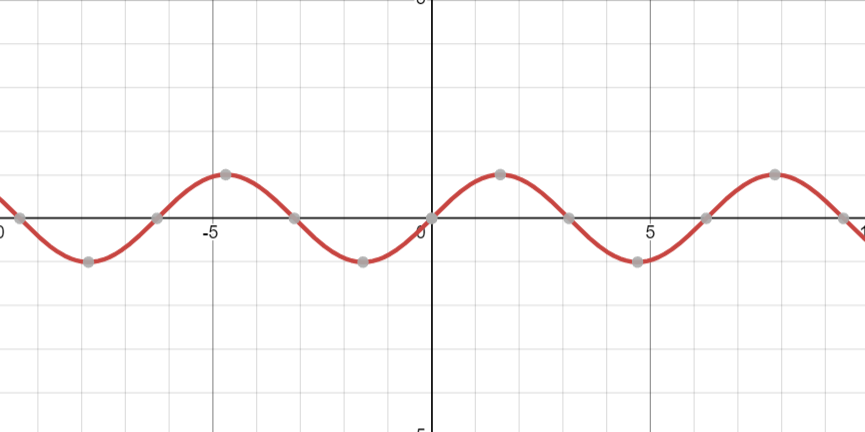
\includegraphics[width=0.7\linewidth]{1.png}\end{center}
Изменим циклическую частоту: $y = \sin{\left(\frac{x}{2\pi}\right)}$: \\
\begin{center}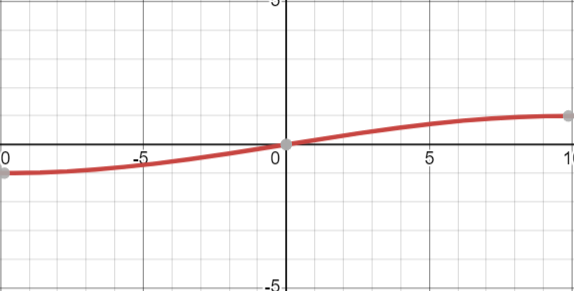
\includegraphics[width=0.7\linewidth]{2.png}\end{center}
Растянем график в 3 раза по OY: $y = 3\sin{\left(\frac{x}{2\pi}\right)}$:
\begin{center}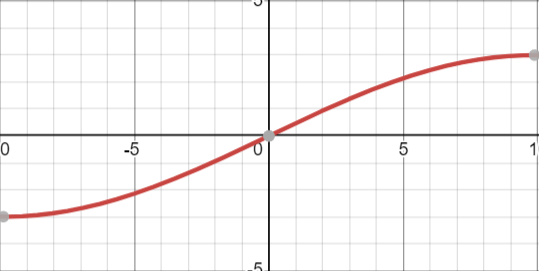
\includegraphics[width=0.7\linewidth]{3.png}\end{center}
Построим график относительно новых осей: 
$y' = y - 5$ и $x' = x - 4\pi$:
\begin{center}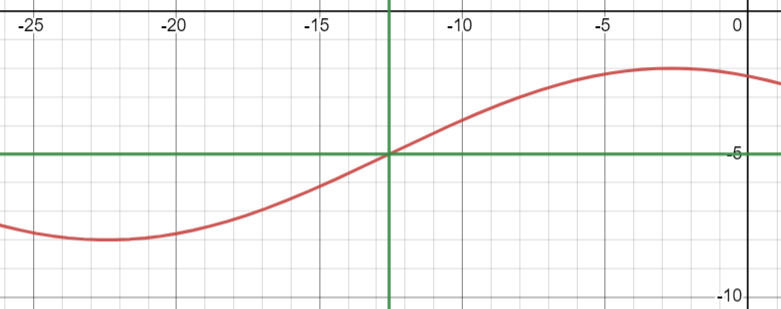
\includegraphics[width=0.7\linewidth]{4.png}\end{center}
В итоге, посредством элементарных преобразований мы получили график функции $y =3\sin{\left(2+\frac{x}{2\pi}\right)}-5$:
\begin{center}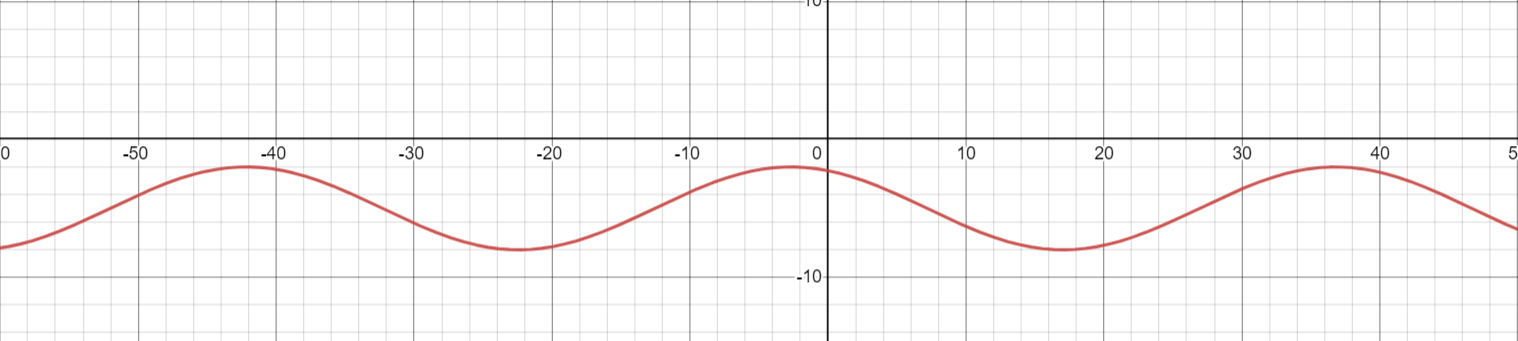
\includegraphics[width=0.7\linewidth]{5.png}\end{center}
\newpage
\[
    2. \hspace{10pt} y =\sqrt{\left(\frac{|6-2x|+x}{10-|5x-15|}\right)^2} = \left|\left(\frac{|6-2x|+x}{10-|5x-15|}\right)\right|
\]
\noindent Раскроем внутренние модули:
\begin{equation*}
    \begin{cases}
        \left|\frac{-x+6}{5x-5}\right|, x < 3 \hspace{20pt} (1)\\
        \left|\frac{3x-6}{-5x+25}\right|, x \geq 3  \hspace{12.5pt} (2)\\
    \end{cases}
\end{equation*}
\noindent Теперь построим $(1)$ и $(2)$ без модулей: \\
{\bf (1):} \\
$\frac{3x-6}{-5x+25}=-\frac{1}{5}+\frac{1}{x-1}$ \\
\noindent Для этого сначала построим базовый график $\frac{1}{x}$: 
\begin{center}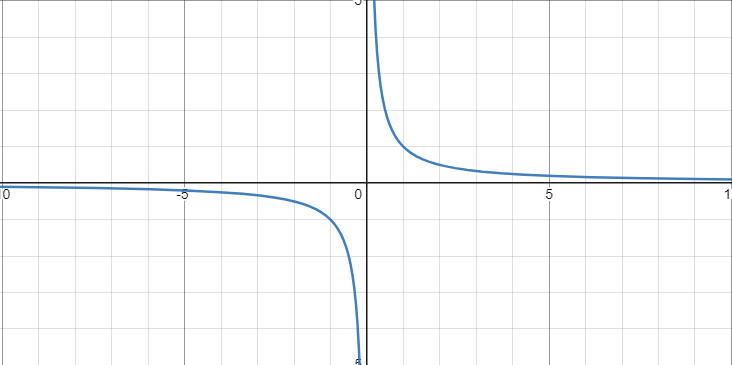
\includegraphics[width=0.7\linewidth]{7.png}\end{center}
После сместим на $+1$ по $x$ и $-\frac{1}{5}$ по $y$:
\begin{center}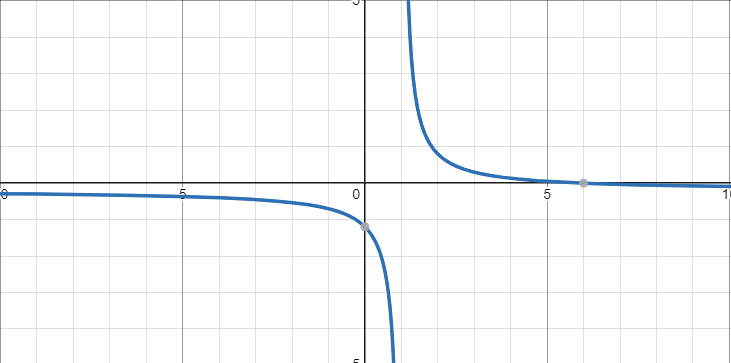
\includegraphics[width=0.7\linewidth]{8.png}\end{center}
\newpage
\noindent Уберем лишнее:
\begin{center}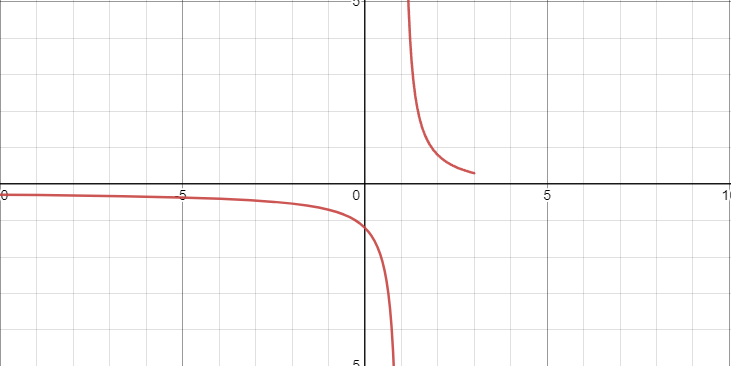
\includegraphics[width=0.7\linewidth]{9.png}\end{center}
Аналогично для {\bf (2):}  \\
$\frac{3x-6}{-5x+25}=-\frac{3}{5}+\frac{9}{-5(x-5)}$ \\
\begin{center}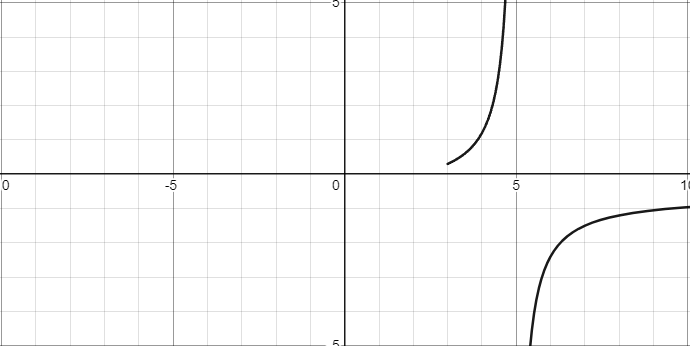
\includegraphics[width=0.7\linewidth]{10.png}\end{center}
\newpage
\noindent Совместим и отразим отрицательную часть относительно оси OX, то есть получим итоговый график:
\begin{center}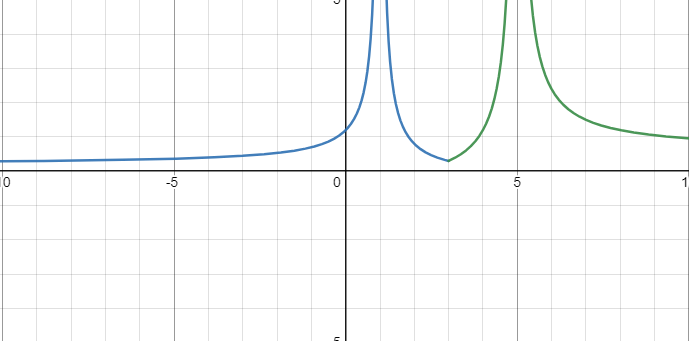
\includegraphics[width=0.7\linewidth]{11.png}\end{center}
\[3. \hspace{10pt} y =\log_4{\left(2+\sqrt{\frac{1}{x}}\right)}\]
График этой функции построим, изучив предварительно ее свойства. \\
Функция определена для $x>0$ и монотонно убывает от $+\infty$ до $0.5$ \\
Построим поочередно графики. Сначала $\frac{1}{x}$ (красная линия), потом  $2+\sqrt{\frac{1}{x}}$ (синия линия), следом     $\log_4{\left(2+\sqrt{\frac{1}{x}}\right)}$ (черная линия):
\begin{center}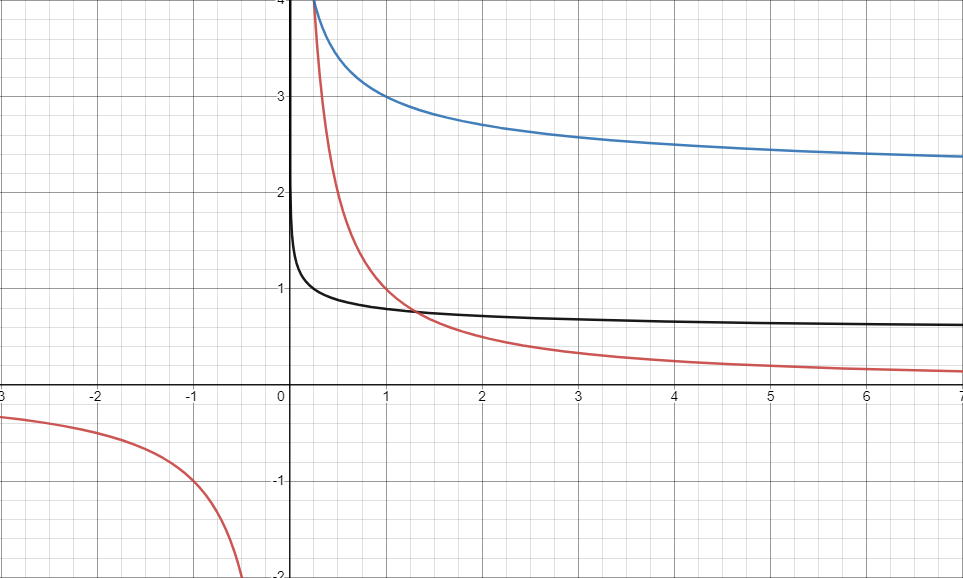
\includegraphics[width=0.7\linewidth]{12.png}\end{center}
